\begin{usecase}{01}{Schermata iniziale}
\usecaseprimaryactors{Utente non autenticato}
\usecasepre{L'utente ha appena avviato l'applicazione.}
\usecasedesc{Vengono visualizzati all'utente alcuni link per accedere a vari siti web legati all'azienda e la possibilità di aprire la pagina di accesso alle funzionalità dell'applicazione.}
\usecasepost{Viene visualizzata la schermata iniziale dell'applicazione.}
\label{uc:UC01}
\end{usecase}

\begin{figure}[!h] 
    \centering 
    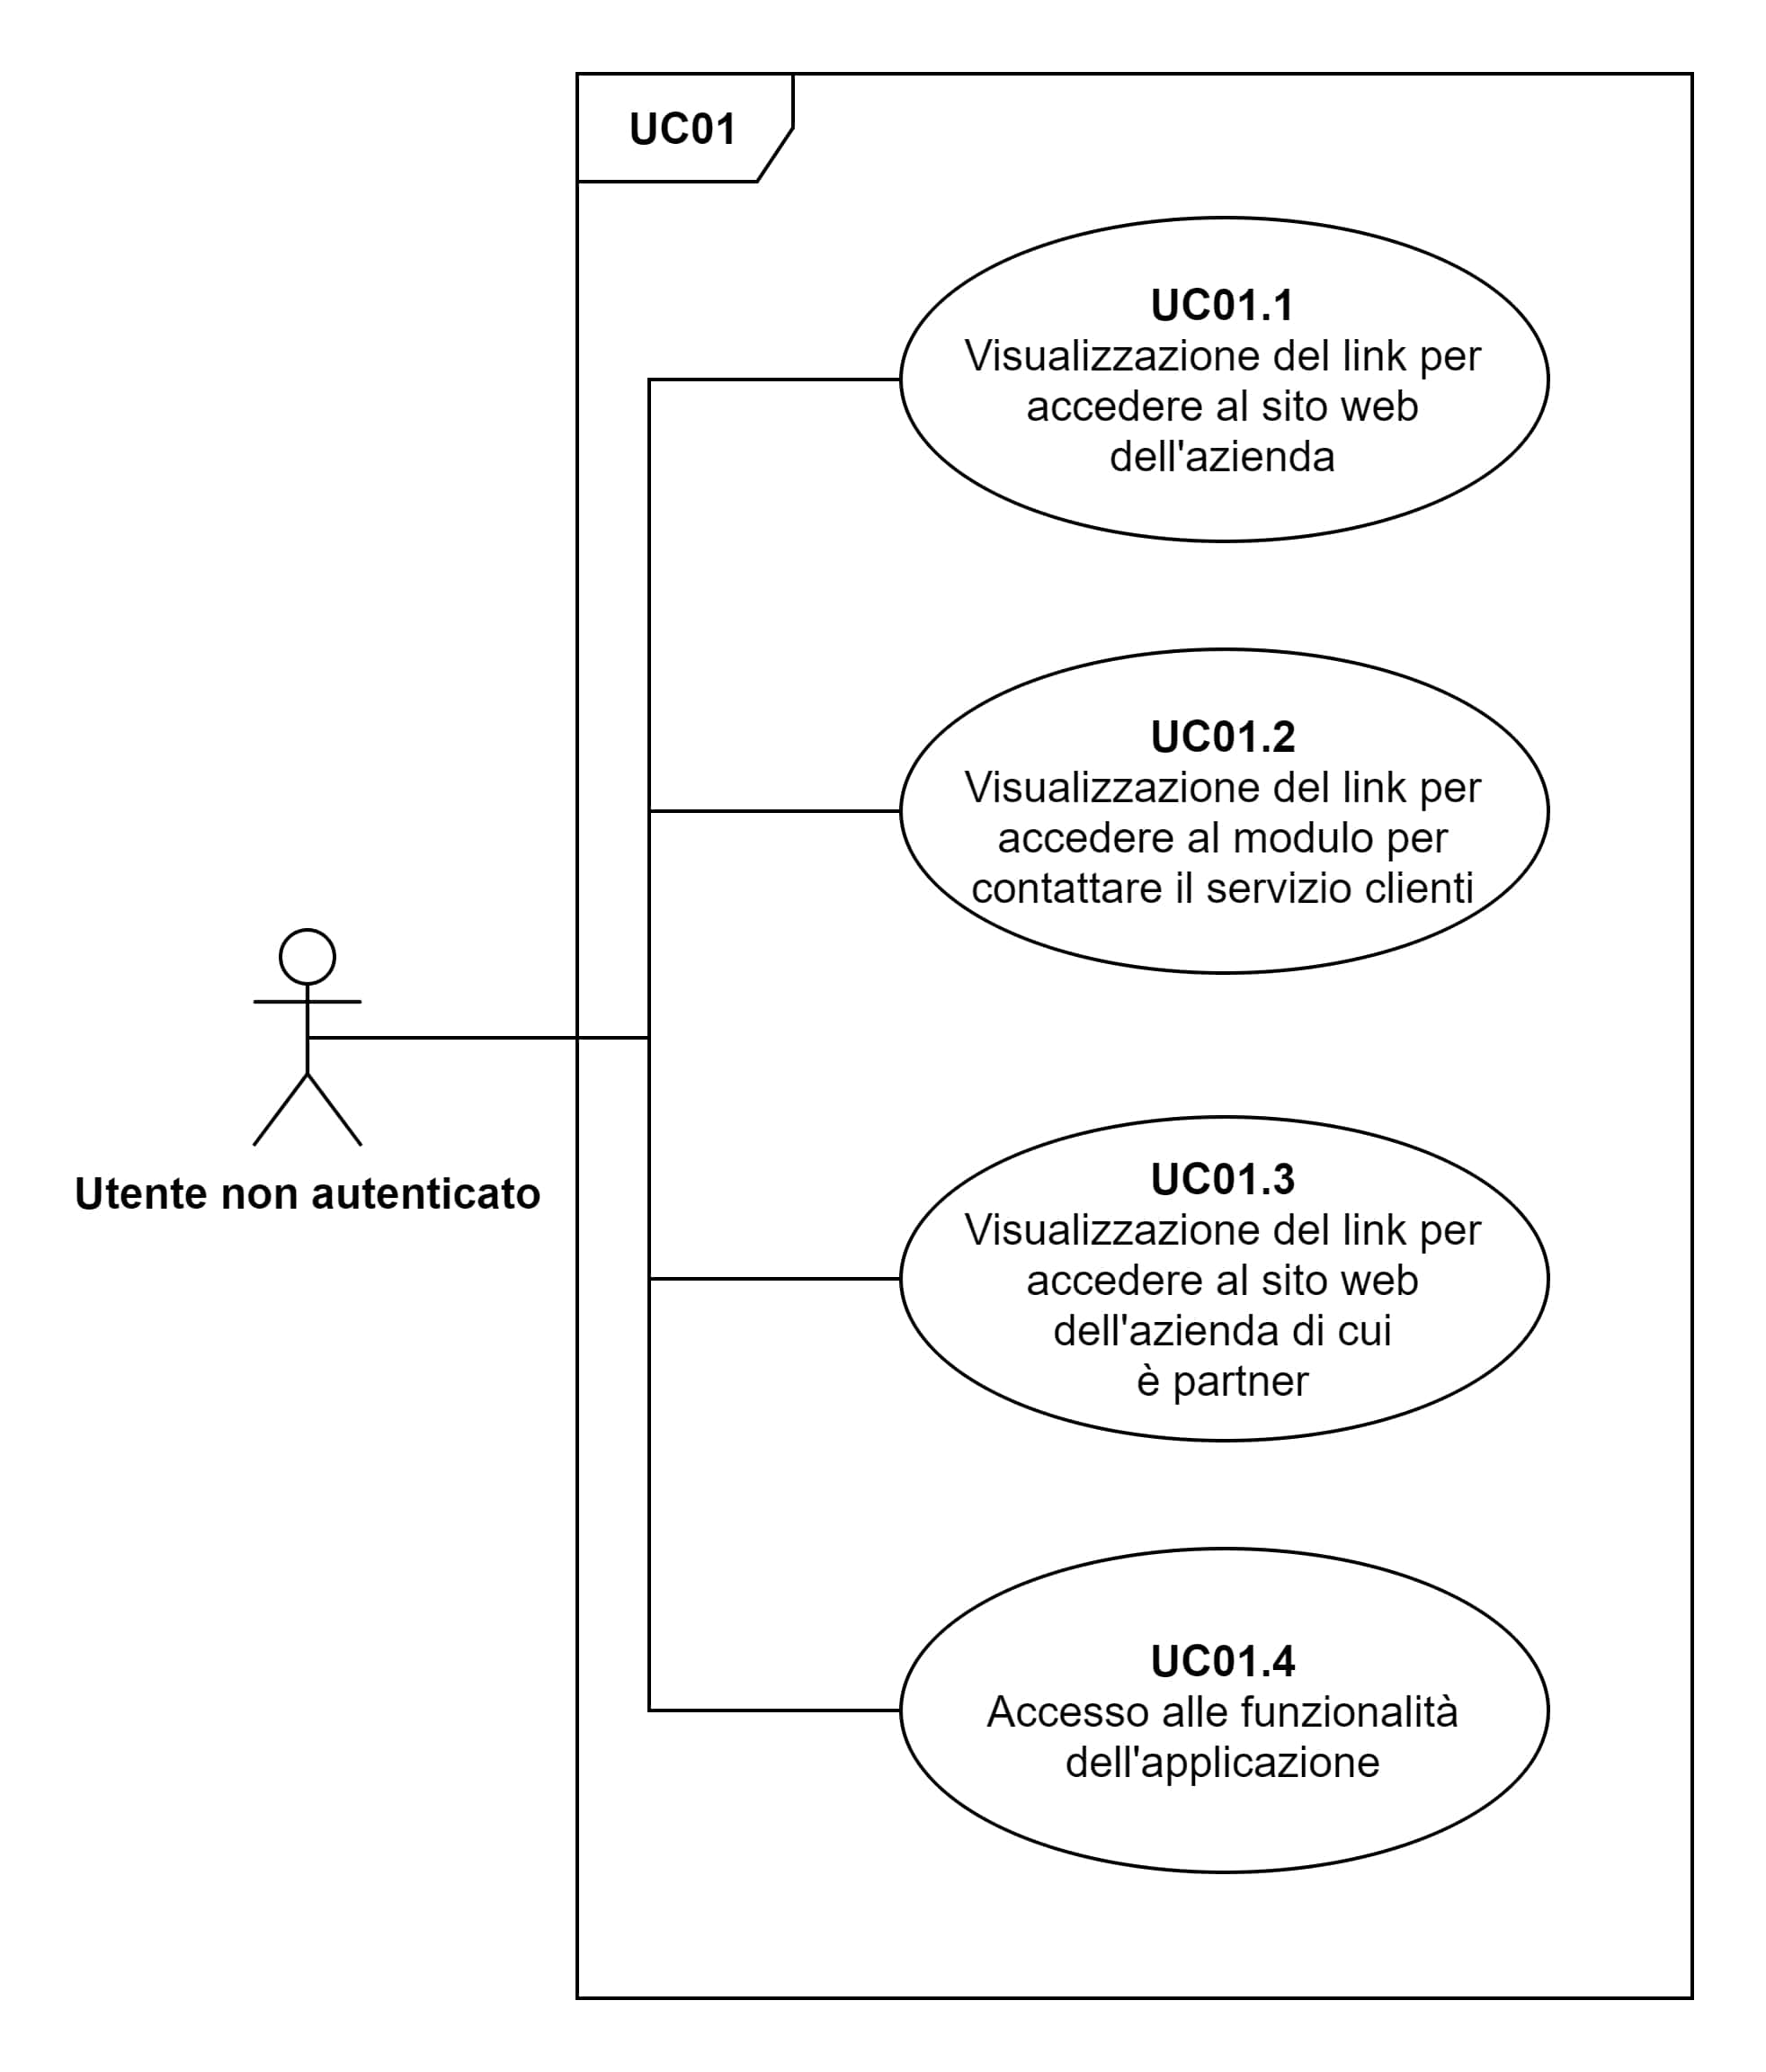
\includegraphics[width=1.0\columnwidth]{appendice-A/uc01} 
    \caption{SMacs - Sotto-casi d'uso di UC01 - Schermata iniziale}
\end{figure}

\begin{usecase}{01.1}{Visualizzazione del link per accedere al sito web dell'azienda}
\usecaseprimaryactors{Utente non autenticato}
\usecasepre{L'utente ha appena avviato l'applicazione.}
\usecasedesc{Viene visualizzato il link per accedere al sito web dell'azienda.}
\usecasepost{Viene visualizzato il link per accedere al sito web dell'azienda.}
\label{uc:UC01-1}
\end{usecase}

\begin{usecase}{01.2}{Visualizzazione del link per accedere al modulo per contattare il servizio clienti}
\usecaseprimaryactors{Utente non autenticato}
\usecasepre{L'utente ha appena avviato l'applicazione.}
\usecasedesc{Viene visualizzato il link per accedere alla pagina web per contattare il servizio clienti.}
\usecasepost{Viene visualizzato il link per accedere al modulo per contattare il servizio clienti.}
\label{uc:UC01-2}
\end{usecase}

\begin{usecase}{01.3}{Visualizzazione del link per accedere al sito web dell'azienda di cui è partner}
\usecaseprimaryactors{Utente non autenticato}
\usecasepre{L'utente ha appena avviato l'applicazione.}
\usecasedesc{Viene visualizzato il link per accedere al sito web dell'azienda di cui è partner.}
\usecasepost{Viene visualizzato il link per accedere al sito web dell'azienda di cui è partner.}
\label{uc:UC01-3}
\end{usecase}

\begin{usecase}{01.4}{Accesso alle funzionalità dell'applicazione}
\usecaseprimaryactors{Utente non autenticato}
\usecasepre{L'utente ha appena avviato l'applicazione.}
\usecasedesc{Viene visualizzato la funzionalità di accesso alla schermata di autenticazione.}
\usecasepost{Viene visualizzato la funzionalità di accesso alla schermata di autenticazione.}
\label{uc:UC01-4}
\end{usecase}